\externaldocument{content/survey}
\externaldocument{content/registration}
\chapter[Omnipresent In-Situ Feedback for Motor Skill Training using AR]{Omnipresent In-Situ Feedback for Motor Skill Training using Augmented Reality \label{chap:omnipresent}}
According to the World Confederation for Physical Therapy, 1,962,741 physical therapists practiced worldwide in 2023. Europe in particular had the highest rate of physiotherapists with 13.5 per 10,000 people~\cite{worldphysiotherapy2023global}. This may be attributed to the fact that 20\% of people globally suffer from chronic pain \cite{treede2015classification}. With computer science advancing, technology can increasingly support therapists and clients alike during therapy. For instance, superimposing virtual content onto the user's perception, as common in \acrshort{mr}, can assist during physical therapy or exercise to facilitate the correct execution of motion \cite{brepohl2023virtual},\cite{campo2021immersive},\cite{diller2022vcb}.

Throughout the literature, we see the use of \acrshort{hmd}s to provide feedback for physical therapy and exercise. On the one hand, these technologies present many challenges to overcome. For example, the first-person perspective of \acrshort{hmd}s limits the user’s view of the user's body parts. On the other hand, \acrshort{hmd}s offer solutions to problems that occur, when providing visual feedback during physical therapy and exercise. For instance, providing visual feedback in a manner that allows users to maintain a neutral head position is challenging. However, if the feedback can only be perceived on a wall-mounted display, users are forced to change their head position, and this --- in the worst case --- inhibits the execution of the correct movements. This can bear serious consequences, such as becoming accustomed to incorrect exercise movement, possibly even leading to injury. For instance, when executing squats correctly, the spine is meant to stay straight. Feedback provided on an \acrshort{rmd} can force the user to bend or twist the neck (and with it the spine) to see the feedback. Therefore, the exercise becomes uncomfortable, the execution can become incorrect, and thus the risk of injury can increase --- especially when performing the exercise with free weights (e.g. barbell). Alternatively, if the exercise is executed correctly and securely, the feedback via \acrshort{rmd} might not be in the user's field of view.

When the motion feedback is provided via an \acrshort{hmd}, the user can execute the movements correctly, comfortably, and non-injuriously. Since the display is mounted on the head, the visual cues can adapt to the head position and the view direction and thus be omnipresent. In this chapter, we present the novel approach \emph{SkillAR} to provide such omnipresent, in-situ, and corrective feedback (as specified in \autoref{sec:feedback}), which adapts to the user's movements, and hence can facilitate an organic and healthy exercise performance. Additionally, we present the results of a user study verifying that SkillAR has no additional disadvantages compared to a conventional screen.

\section{Point of View in Motor Feedback\label{sec:omnipresent:POV}}
Considering motion feedback, the \emph{\acrshort{pov}} plays an important role. A first-person perspective (\autoref{fig:POV:AR}, right) provides an immersive and natural viewpoint, as we usually experience the world from this angle. However, the foreshortening deriving from this perspective can make it difficult to perceive the spatial positioning of limbs. Furthermore, some body parts, like the back, can simply not be observed from this limited viewpoint. 
Optical see-through \acrshort{hmd}s (as are used in this chapter) always provide a natural first-person perspective in addition to any other superimposed feedback types.

Alternatively, a common way to display motion feedback is a third-person perspective (\autoref{fig:POV:AR}, left). This gives the user an overview of his or her body in space. The relation of all limbs becomes clear and deviations from the correct form can be adjusted accordingly. Therefore, Rymal and Ste-Marie~\cite{rymal2009dsm} discovered that an exocentric view of an exercise could help athletes improve their ability to mentally visualize the motion, which can lead to learning new skills or improving performance~\cite{white1998ida}. Moreover, we elaborated in \autoref{chap:visualCueSurvey} that a third-person view is predominantly used in current literature when providing visual feedback for motor skills.

\begin{figure*}[b!]
	\centering
	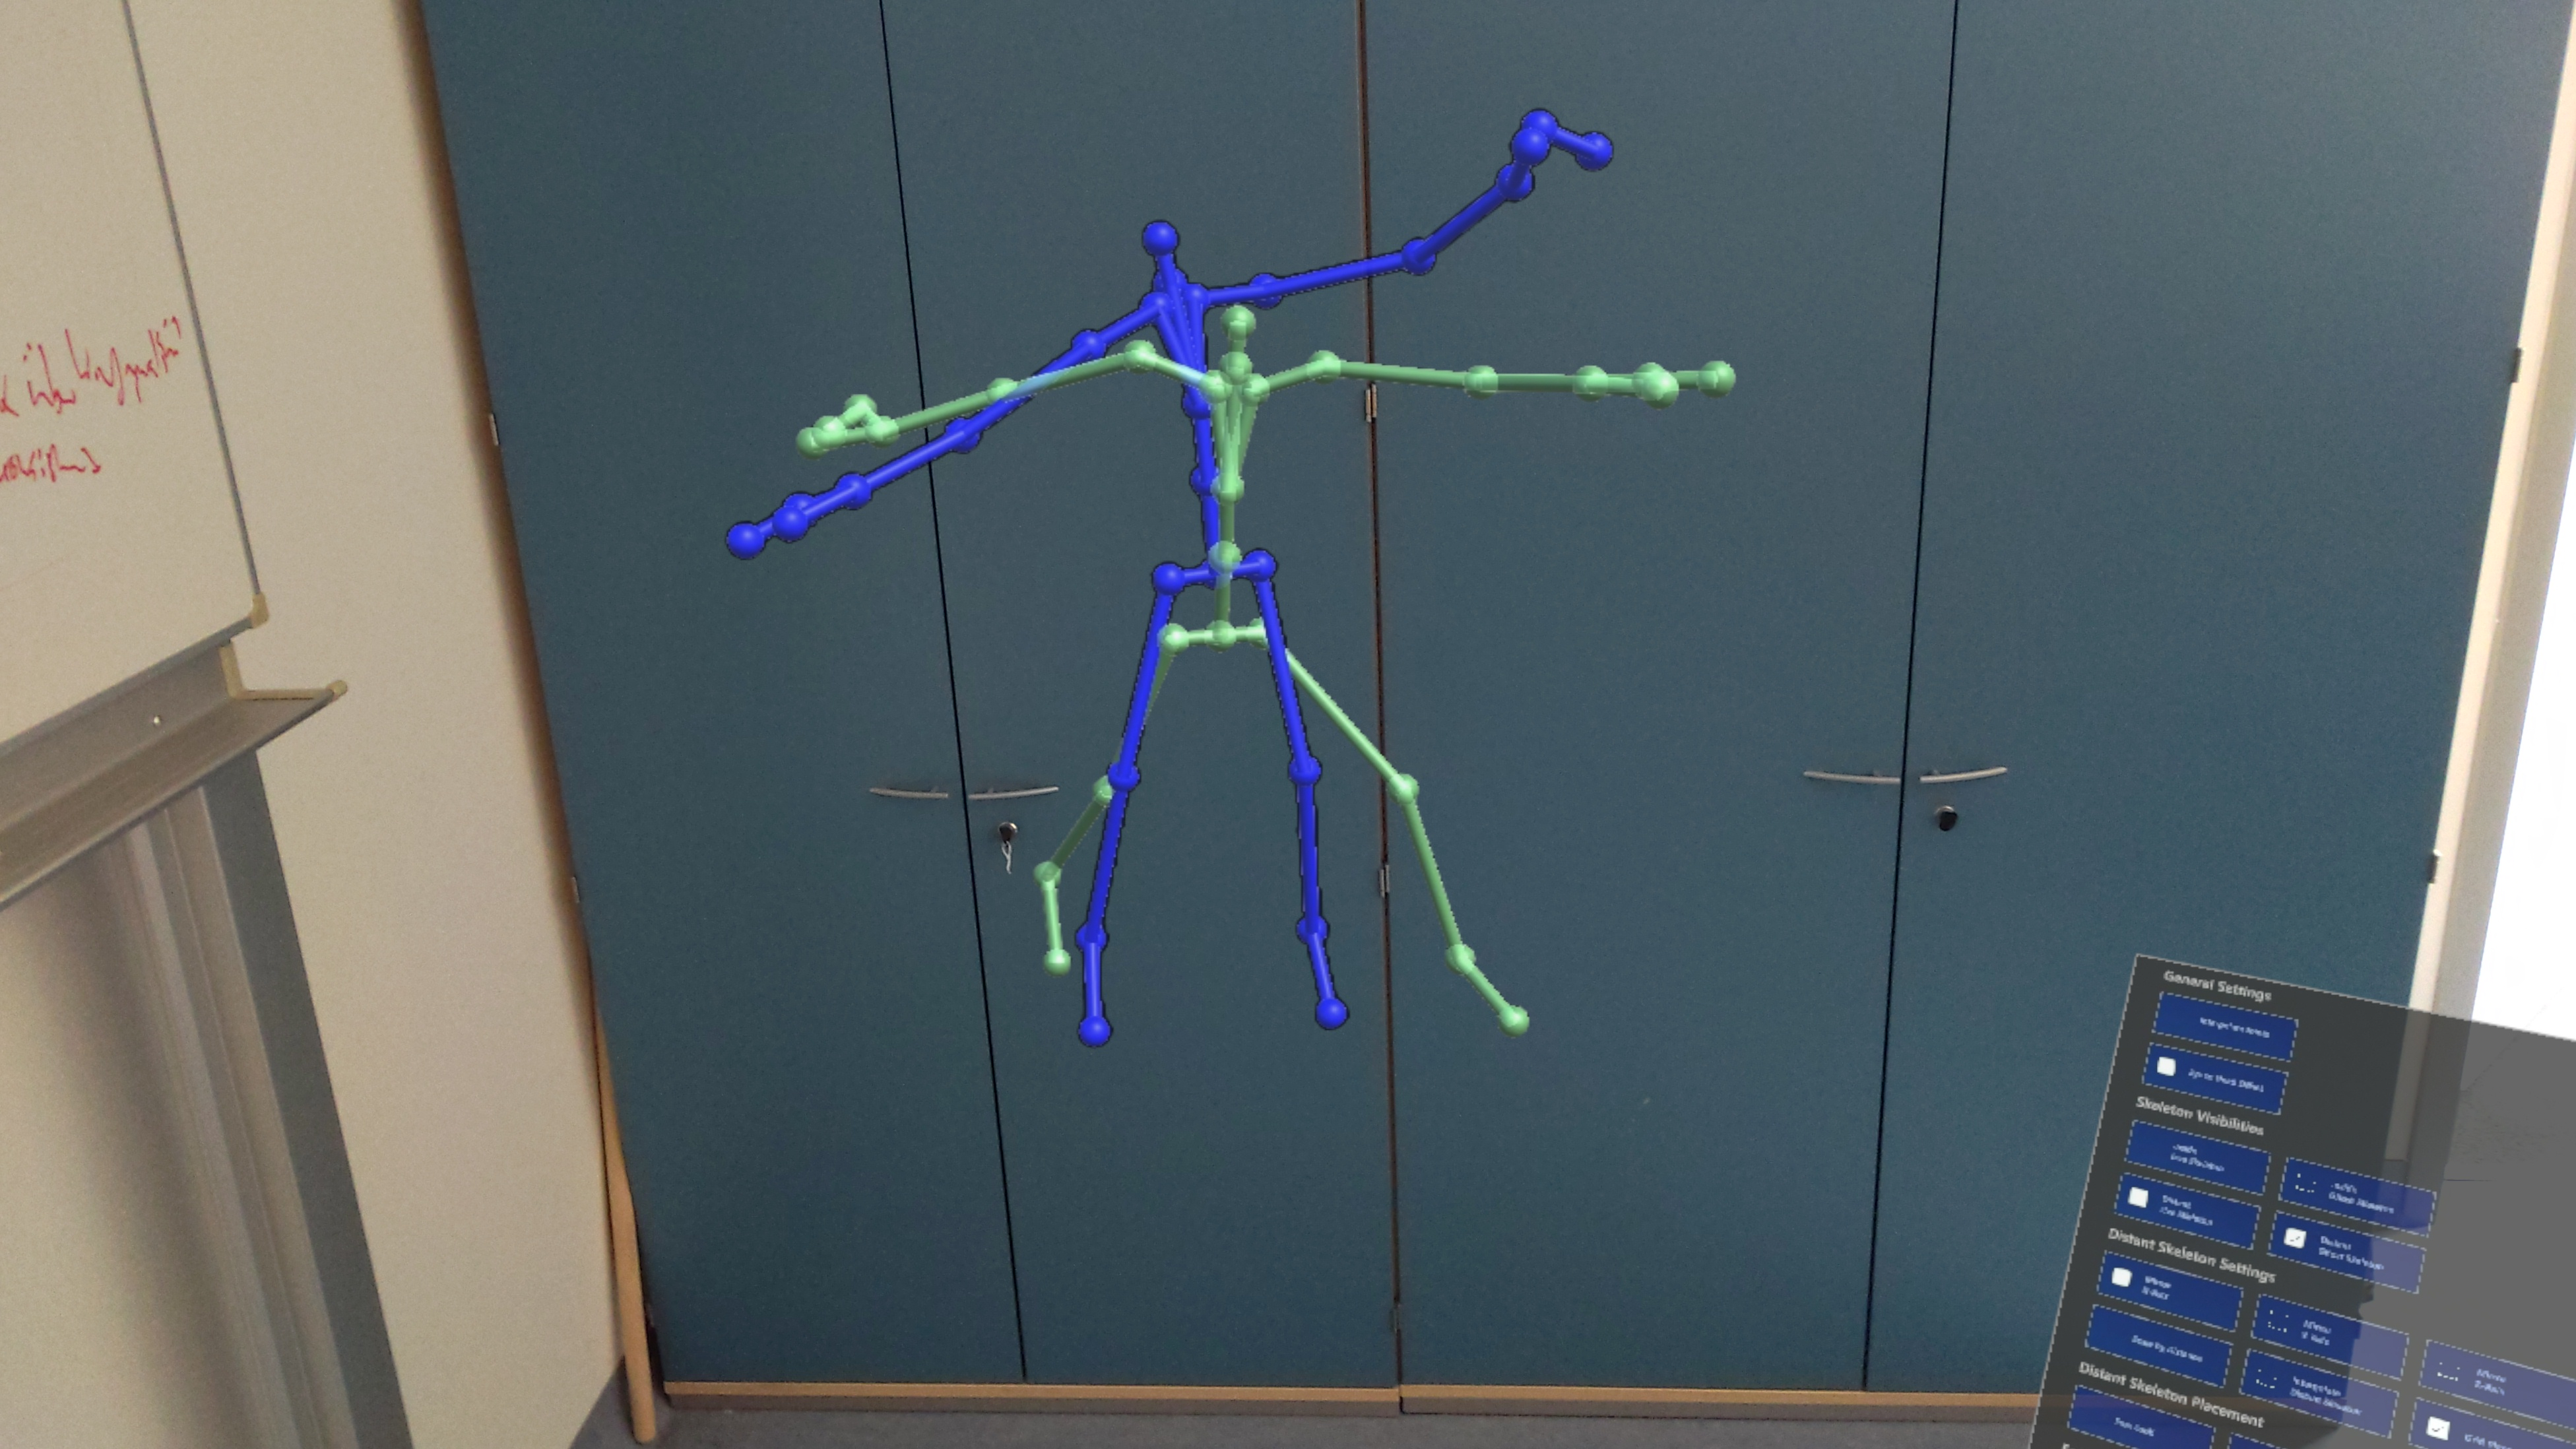
\includegraphics[width=0.49\linewidth]{pictures/ExocentricAR.jpg}\hfill
	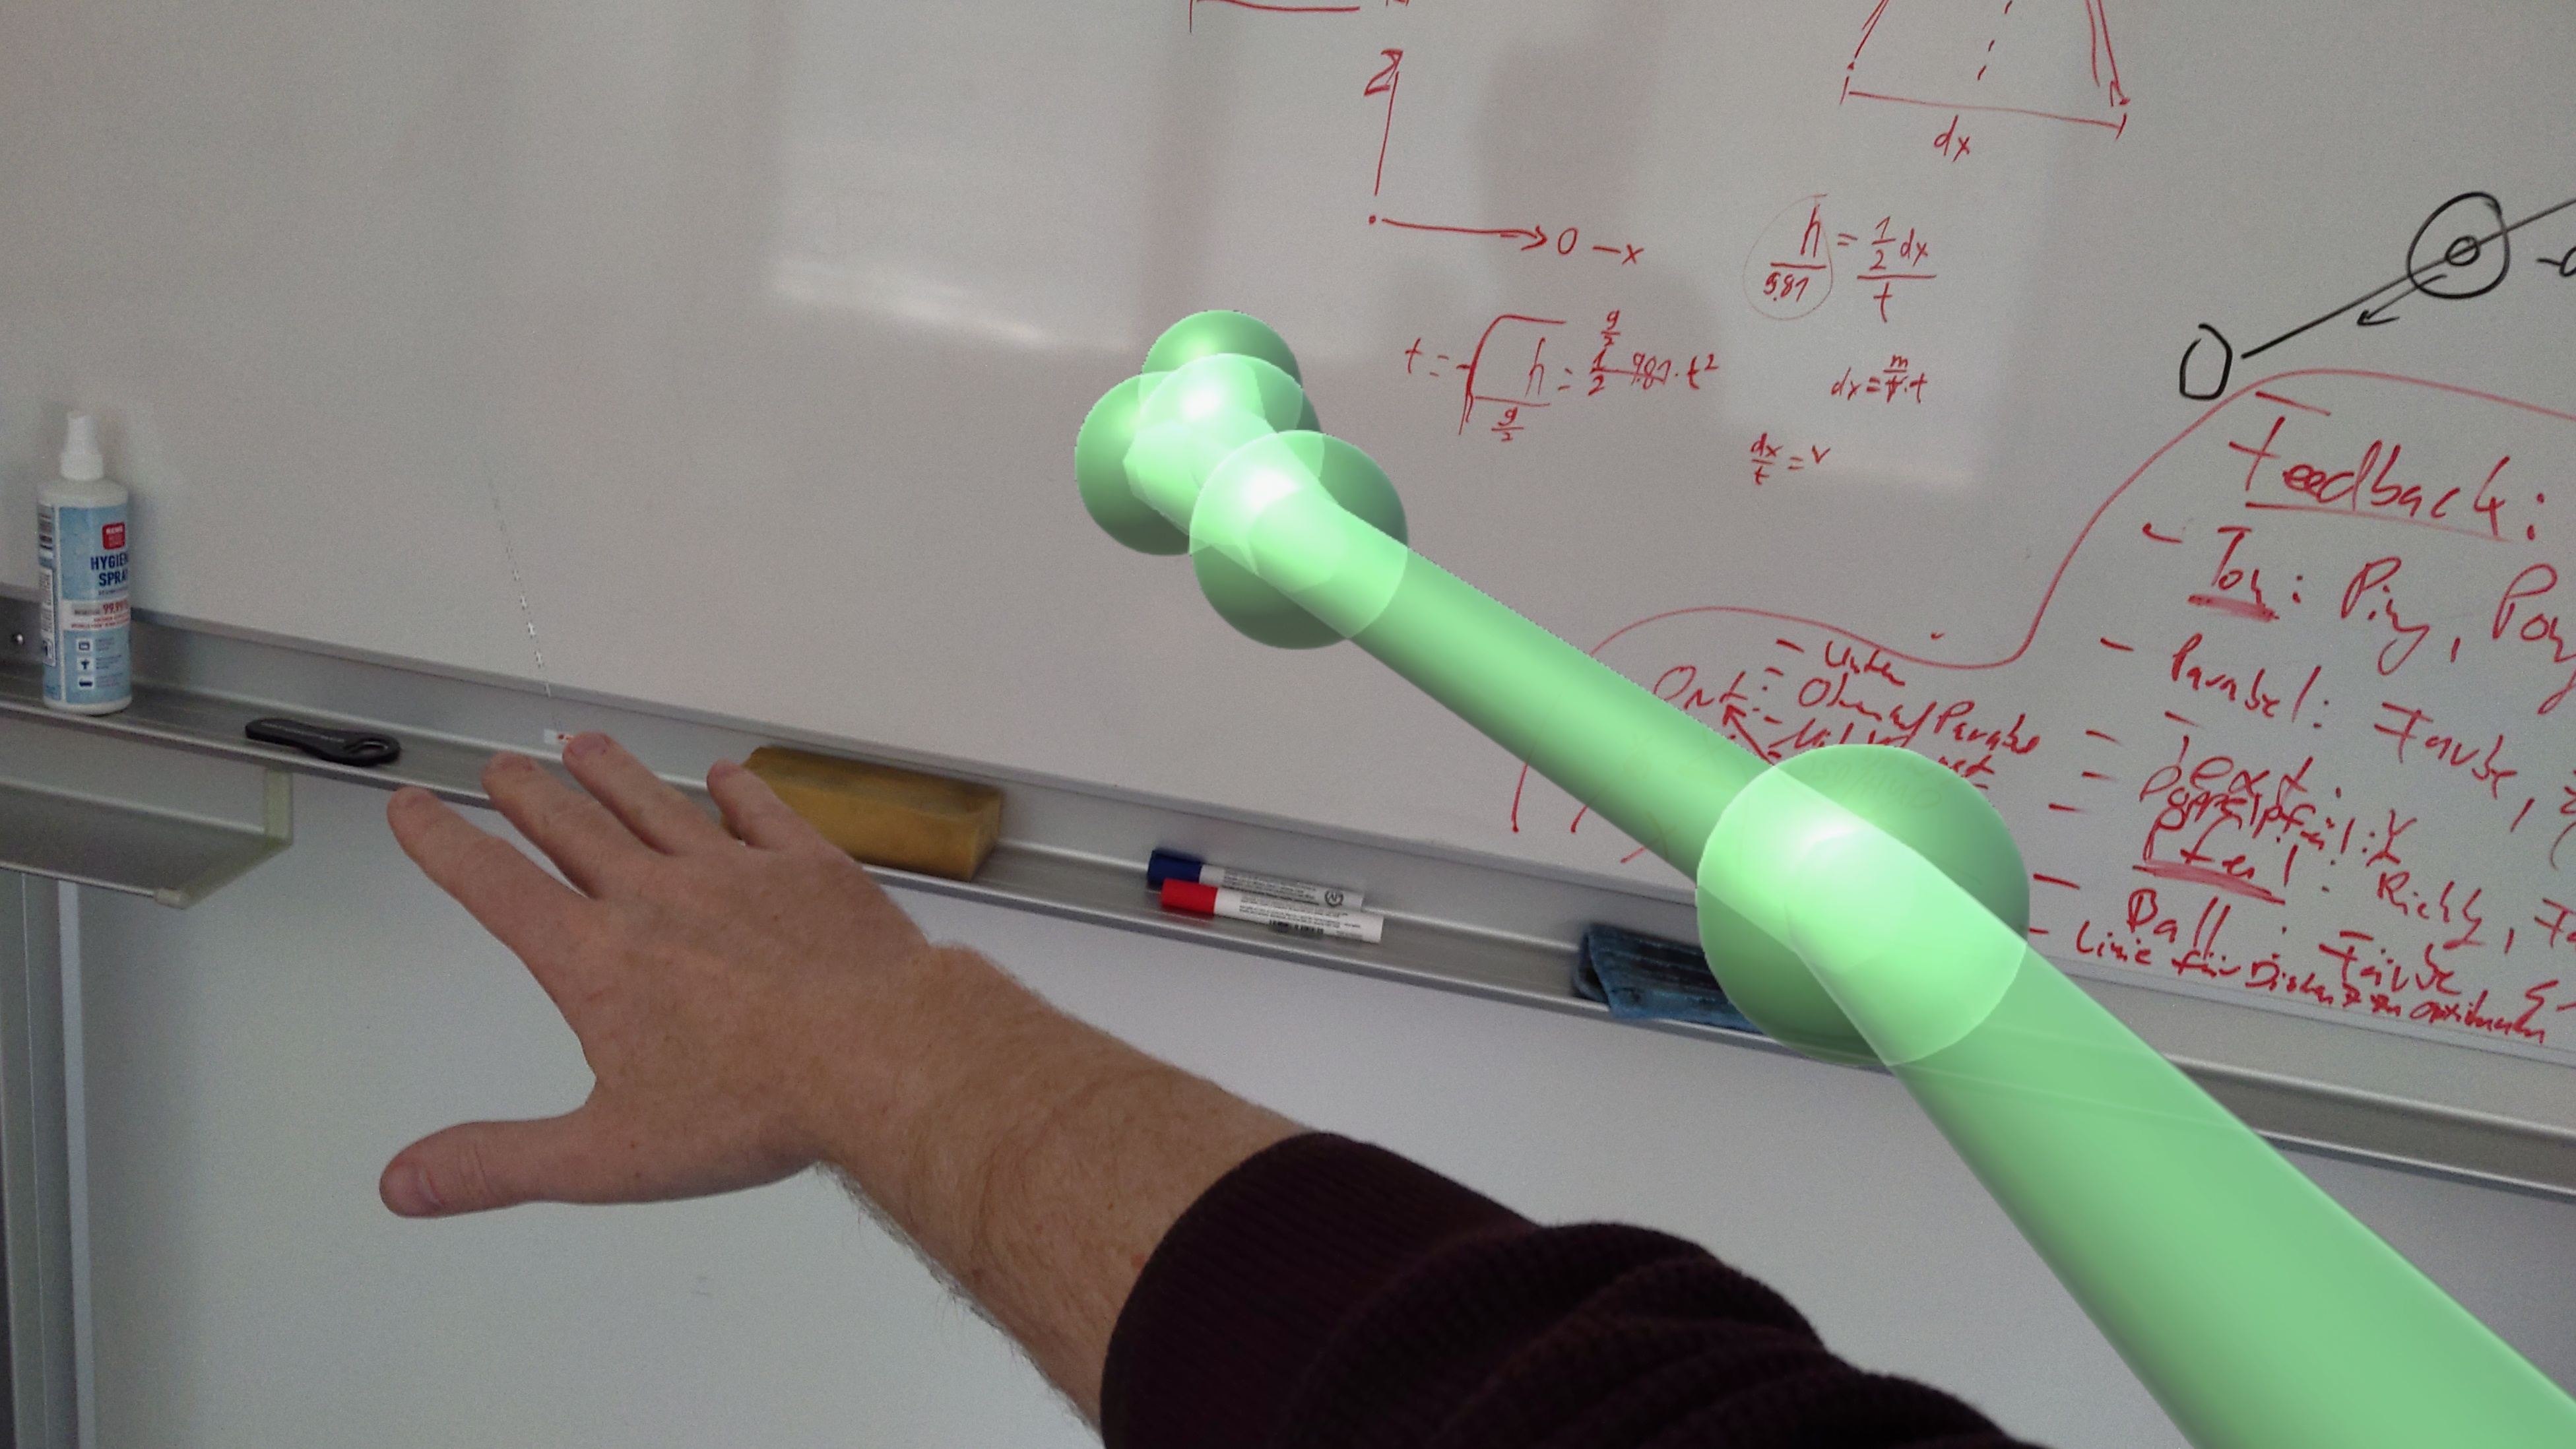
\includegraphics[width=0.49\linewidth]{pictures/EgocentricAR.jpg}
	\caption[Examples of exocentric and egocentric motion feedback in \acrshort{ar}.]{Examples of exocentric (left) and egocentric (right) motion feedback in augmented reality. The possible target movement is in both cases represented by a green avatar. Compare to the stylized illustration in \autoref{fig:POV}.}
	\label{fig:POV:AR}
\end{figure*}

Furthermore, for facilitating a user-friendly and intuitive viewpoint selection \autoref{sec:considerations} provides additional considerations. Moreover, with the methods presented in \autoref{sec:methViewCalc}, it is possible to calculate an optimized viewpoint of the exocentric motion feedback. However, this exceeds the scope of this chapter.

\section{Common Visual Feedback Technologies} %Methods?
The most common tool to obtain a full-body view (i.e. third person / exocentric as seen in \autoref{fig:POV:AR} and explained in~\autoref{sec:omnipresent:POV}) is the mirror. Ballet dancers and their instructors have utilized mirrors to acquire simple visual feedback since the 19th century~\cite{desmond1997mim}. Likewise, mirrors are to be found in fitness studios and physiotherapy studios all over the world. Furthermore, it is possible to enhance the natural feedback of the mirror with technology. Such enhancements often lead to smart mirrors, which can assist with correct exercise execution (e.g. \cite{kim2020rtm}, \cite{park2021ued}). Moreover, some approaches use the mirror metaphor in a \acrshort{vr} setting to create an intuitive feedback system (e.g. \cite{waltemate2016tlp}, \cite{huelsmann2019ssp}). These so-called \emph{virtual mirrors} are additionally often used to increase the sense of embodiment \cite{inoue2021virtual}, \cite{gonzalesfranco2010contribution}.

Equally important in recent research are conventional displays. Especially in connection with mobile devices or computers, displays are able to provide visual feedback for motor skill training. In some instances, \acrshort{rmd}s mimic the function of mirrors. These approaches are commonly described as \emph{augmented mirrors}. For example, Anderson et al.~\cite{anderson2013youmove} visualize an actual avatar and a target avatar on a room-scale display in addition to a camera stream. Likewise, Trajkova et al.~\cite{trajkova2018ttb} provide feedback as a mirrored camera stream with superimposed feedback. As we showed in \autoref{chap:visualCueSurvey}, augmented mirrors are a prevalent motor feedback approach in the literature. 

\section{Related Work}
Several approaches addressed the limitations of the first-person perspective in \acrshort{hmd}s as described in \autoref{sec:omnipresent:POV} when providing motion feedback. For example, Chua et al. \cite{chua2003tpt} provided feedback for tai chi displaying several redundant exocentric feedback avatars around the user. This solved the visibility issue when moving the head, i.e. changing the view direction in the first-person perspective in \acrshort{vr}. Additionally, the approach explored different feedback methods, like a single teacher or superimposed wireframe feedback.

Likewise, Han et al. \cite{han2017mtc} utilized multiple coaches fixed in space and oriented circularly around the user. However, they transferred the idea into \acrshort{ar}. In addition to the redundant instructors (see also \autoref{sec:instructor}), a drone was automatically navigated to record the user. This video stream was then displayed in \acrshort{ar}, mimicking a mirror. As a result, the user could see a coach executing the target movement in every horizontal direction juxtaposed with the mirror image. However, while this approach might be well-matched for the use case of tai chi, feedback would not be visible in exercises where the view is naturally directed to the ground (e.g. planks, push-ups) or the ceiling (e.g. sit-ups, bench press).

Yan et al.~\cite{Yan2015oma} solved the issue of a limited first-person perspective by juxtaposing the \acrshort{hmd} video pass-through with the video stream of an external camera. This image was cropped at the silhouette to blend with the surroundings and create a cohesive \acrshort{mr} experience. Although the approach provided an exocentric feedback of the body, the functionality was limited by the position and view direction of the physical camera.

In contrast to the previously mentioned works, Kawasaki et al.~\cite{kawasaki2010cst} included the perspective of another person by superimposing the user's view with the video see-through stream of an \acrshort{hmd}. As a result, the user could see if his or her motions corresponded with the instructor's. This enabled skill transmission in a user study. A similar approach was taken by Kasahara et al.~\cite{kasahara2016pe}, who also included another person's perspective in an \acrshort{hmd}. In contrast to the previous work, the two perspectives were juxtaposed. The two approaches enhance the egocentric perspective, therefore they are well suited for skill training mostly involving the hands, like diabolo juggling~\cite{kawasaki2010cst} or drawing~\cite{kasahara2016pe}. However, they lack an exocentric perspective and hence an overview of the body, making feedback for whole-body exercises impossible.



In addition, Ikeda et al. \cite{ikeda2018arb} displayed stationary small-scale (1:4) avatars in real-time during the motion and true-scale models during playback feedback. As the system was built specifically for golf swings and players look downwards during swings, the small-scale avatar could be seen during the exercise performance. Afterward, when replaying a recorded exercise, the view was no longer restricted by the exercise. Consequently, the avatar was displayed in true-scale. Although the avatar could be seen well when performing a golf swing, there are some exercises, for which providing feedback with this system would prove difficult. In particular, difficulties arise for exercises where rotating the view direction on the horizontal plane or an almost vertical view direction is necessary.

Lastly, Hamanishi et al. \cite{Hamanishi2019avu} developed a system that enables the user to view his or her motions from all sides. This was achieved by giving the motion-captured avatar a fixed direction in space. Consequently, the user can walk around it, viewing it comprehensively. The two participants of the qualitative user study seemed to receive the system well. However, it might not be sufficient for all forms of exercise. For example, the feedback might irritate users during exercises where the view direction changes a lot (e.g. sit-ups, torso rotations). Furthermore, the system did not provide a target movement for the user to imitate. Hence, the system does not qualify as \emph{corrective feedback} (see \autoref{sec:feedback}), which is the focus of the work at hand.

\section{Omnipresent Feedback}
This section will explain the SkillAR system in detail. First, \autoref{sec:overview} and \autoref{sec:register} will provide information about the hardware used and the nature of the feedback displayed. This should give the reader an understanding of the whole system. Our main contributions lie in the combination of methods found in \autoref{sec:transformation} to ensure the omnipresence of the feedback.

\subsection{System Overview \label{sec:overview}}
\begin{figure}[b!]
	\centering
	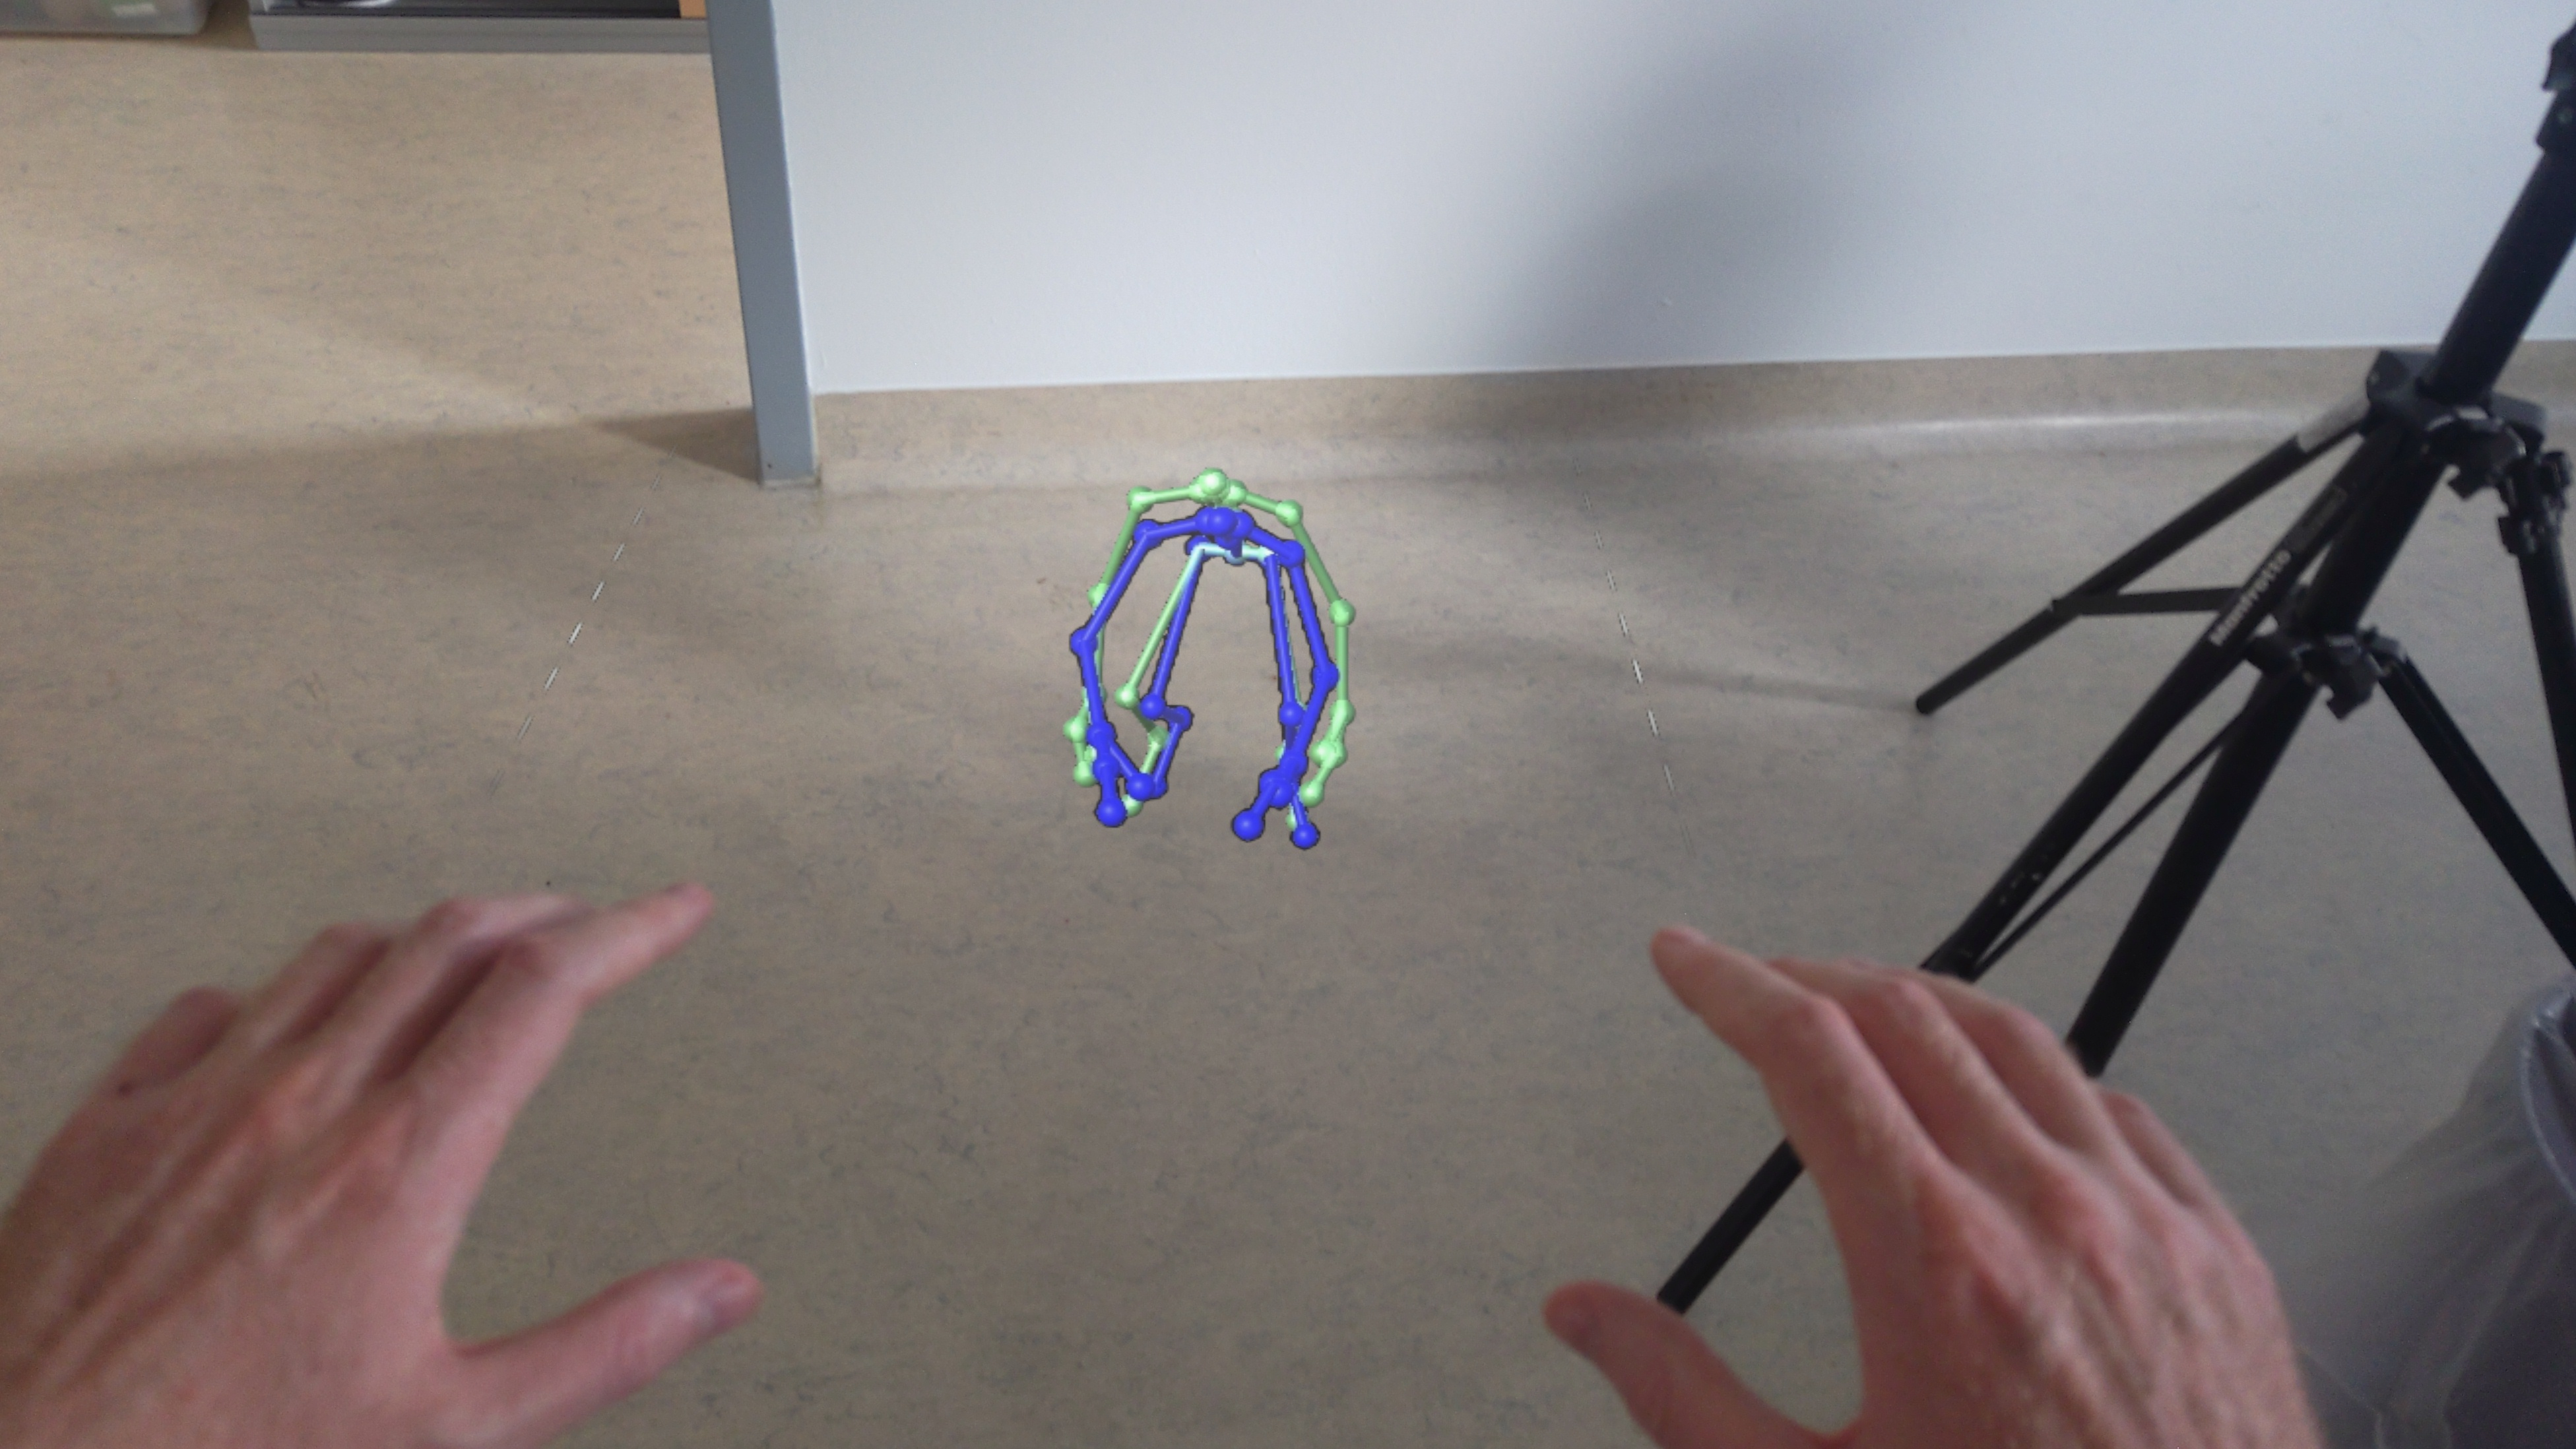
\includegraphics[width=\linewidth]{pictures/HoloLensScreenshot.jpg}
	\caption[Screenshot of the motor feedback provided by SkillAR via \acrshort{hmd}.]{Screenshot of the egocentric motor feedback provided by SkillAR via \acrshort{hmd}. \label{fig:screen}}
\end{figure}
In order to provide visual feedback for motions and in particular exercises, it is necessary to capture the limb positions in space over time. For this reason, we used a 3D camera, which extracted joint coordinates from a recorded point cloud. Consequently, a skeleton-like avatar as seen in \autoref{fig:screen} could be constructed on the \acrshort{hmd}, showing the executed motion in real-time. In addition to the current motion, we superimposed a recorded movement, which represents an ideal execution of the movement. As a result, the user can now correct the motion following the provided feedback. In addition to superimposition, there are further possibilities to display comparative visuals as analyzed by L'Yi et al.~\cite{lyi2021comparative}. Varying avatars and visual cues could impact how users perceive the feedback and therefore yield different results in a user study as conducted in \autoref{sec:evaluation}. However, evaluating different visual cues and avatars would exceed the scope of this paper.


\subsection{Avatar Registration \label{sec:register}}
As described in \autoref{chap:registration}, the registration of superimposed avatars is no trivial subject. Depending on where the actual and target avatars are registered, the visualization is perceived as intuitive or irritating by the user.
\begin{comment}
\begin{figure*}[h!]
	\centering    \subfloat{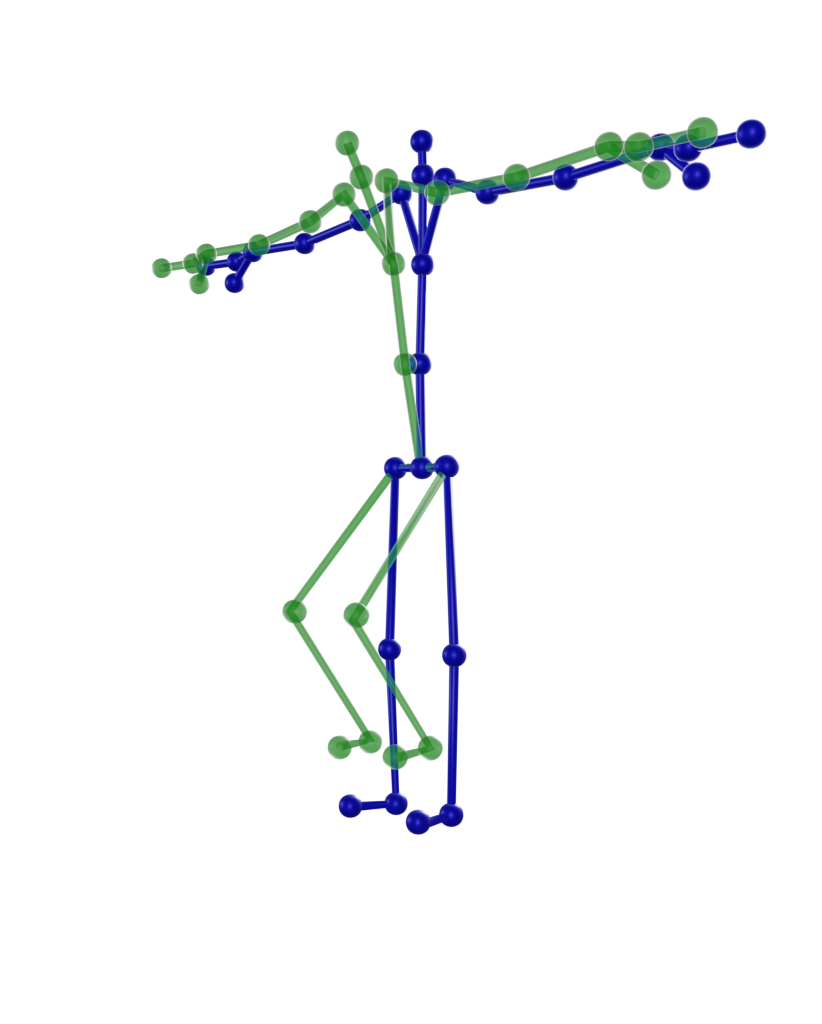
\includegraphics[width=0.5\linewidth]{pictures/pelvisRegistration.png}\hfill}
	\subfloat{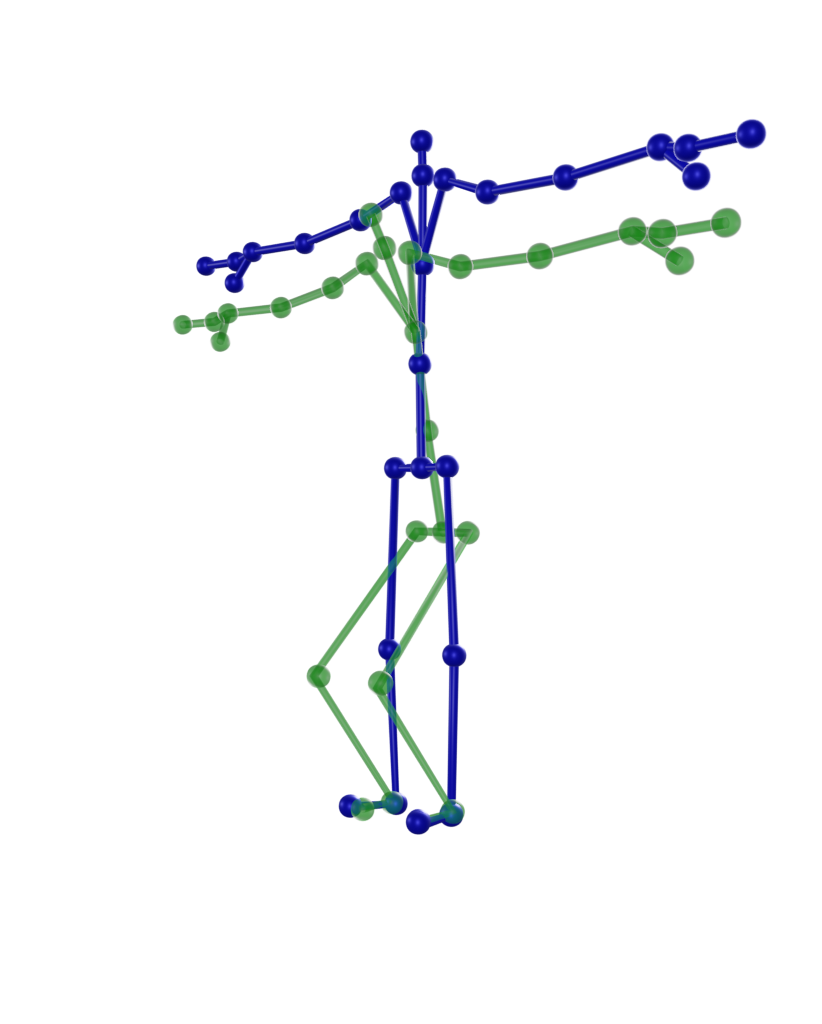
\includegraphics[width=0.5\linewidth]{pictures/footRegistration.png}\hfill}
	\caption[Example of different methods registering squatting skeletons.]{The reference (in green) is performing the ideal exercise --- in this case a squat --- while the actual avatar is neutrally standing. The result of registering at the pelvis (left) looks as if hovering and can potentially be irritating to the user. In this case, it might be preferable to register the avatars at the foot or the ground. \label{fig:registration}}
\end{figure*}
\end{comment}


\begin{figure*}[t!]
	\centering
	\subfloat[\centering Standing]{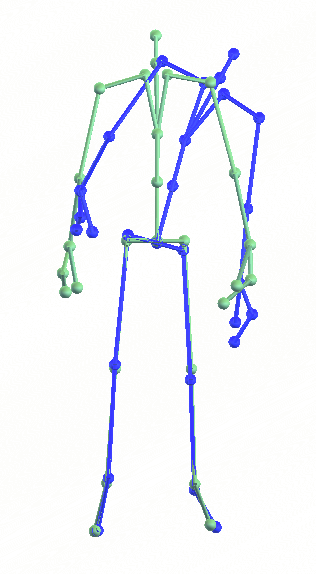
\includegraphics[width=.13\linewidth]{pictures/Standing.png}\hfill}  
	\subfloat[\centering Jumping\\Jack]{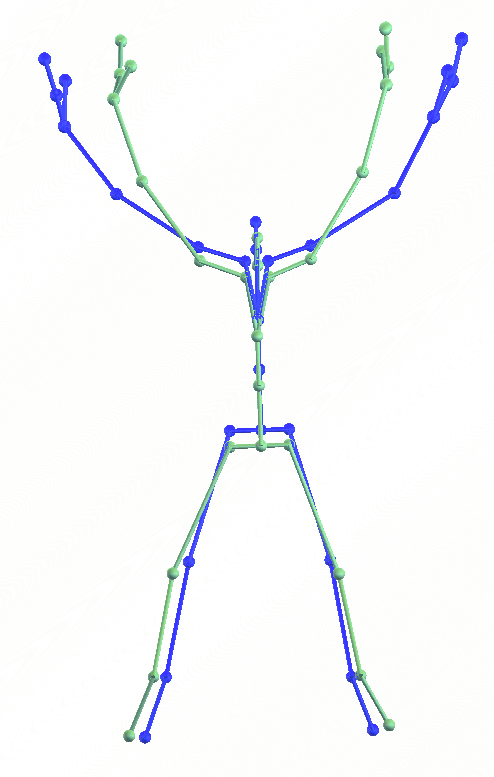
\includegraphics[width=.15\linewidth]{pictures/JumpingJack.png}\hfill} 
	\subfloat[\centering Plank]{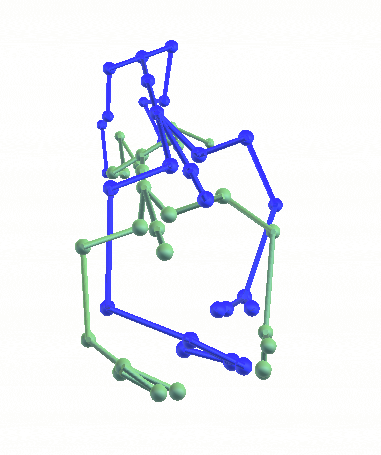
\includegraphics[width=.15\linewidth]{pictures/Plank.png}\hfill} 
	\subfloat[\centering Squat]{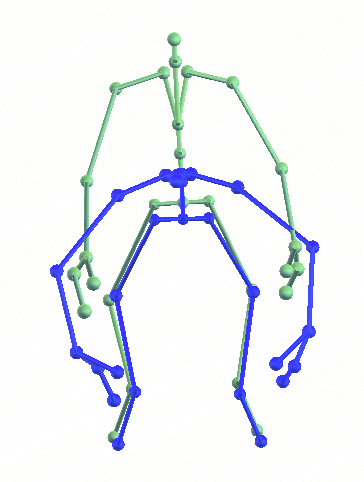
\includegraphics[width=.15\linewidth]{pictures/Squat.png}\hfill} 
	\subfloat[\centering Torso\\Rotation]{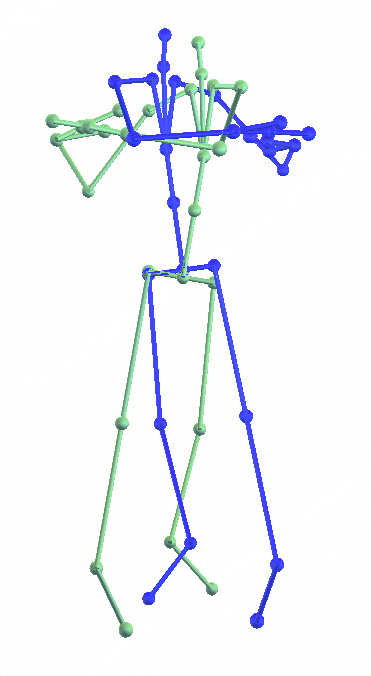
\includegraphics[width=.13\linewidth]{pictures/TorsoRotation.png}\hfill}
	\subfloat[\centering Warrior II]{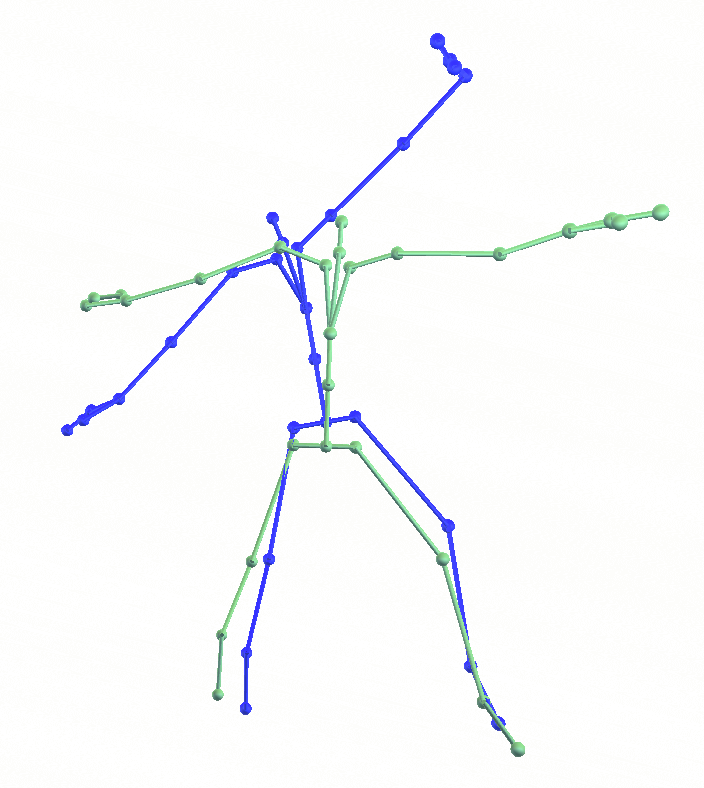
\includegraphics[width=.22\linewidth]{pictures/WarriorII.png}\hfill} 
	\caption{Example exercises with deviations as described in \autoref{sec:design}.}
	\label{fig:exercises}
\end{figure*}

Consequently, in our work, we fixated the actual avatar and matched the horizontal position of the pelvises. For the vertical position of the target reference avatar, we matched the lowest feet position of both avatars, considering that it should be on the ground since we did not include exercises that involved jumping or hanging (see~\autoref{fig:exercises}), as we wanted the exercises to be feasible for a large group of people. Considering rotation, the orientation of the actual pelvis joint was transferred to the target pelvis joint. The registration methods closely align with the approach presented in \autoref{chap:registration}. For an in-depth analysis of avatar registration, see the corresponding chapter.

Additionally, the target avatar had to be scaled bone-wise to match the anatomy of the user. Otherwise, it would be impossible for the user to mimic poses recorded by someone else, as limbs cannot be stretched or compressed. If the same individual records the ideal and actual execution, this step can be skipped. Furthermore, the avatars were mirrored horizontally, as this makes it easier to take the displayed pose and increases embodiment as stated, for example, by Raffe and Garcia~\cite{raffe2018combining}.

\subsection{Feedback Transformation \label{sec:transformation}}
Because SkillAR intends to provide omnipresent in-situ feedback, avatar transformation in space is crucial. Utilizing the orientation of the \acrshort{hmd} in space and the information we have of the body and surroundings, we can transform the feedback to adapt to the head movement during different exercises and to facilitate a better understanding of the feedback itself. Internal pilot studies have shown various important aspects that we will illustrate in the following.

\textbf{Placement:}
The stereoscopic display of the \acrshort{hmd} makes it possible for the user to perceive the avatars in space. Consequently, placing the avatars in relation to the actual surroundings of the users helps enhance the interpretation of the feedback. For this purpose, we use the view direction $\vec{v}$ of the \acrshort{hmd} to place the avatar. An intuitive way of placing would be to position the avatars' feet at the intersection of $\vec{v}$ with the floor plane. However, this would often lead to the avatar only taking up the upper half of the user's field of view. Instead, the avatars' pelvis represents an adequate approximation of the body center. Yet, we can not place the avatar with its pelvis is at floor height, as the feedback would appear too low (partially below ground) and hence be irritating. Instead, we constructed a plane $P$ horizontally through the user's pelvis. The avatars (registered as described in \autoref{sec:register}) were then positioned by placing the pelvises at the intersection of $\vec{v}$ and $P$ as seen in~\autoref{fig:positioning}. Using the pelvis orientation as an indicator for the forward direction of the avatar, the feedback was rotated around the vertical axis, so it faced the virtual camera and thus, the user. This supports the mirror metaphor and hence user guidance as described in~\autoref{sec:register}. The steps above ensure that the feedback is visible in any view direction, i.e. omnipresent.

\begin{figure}[b!]
	\centering
	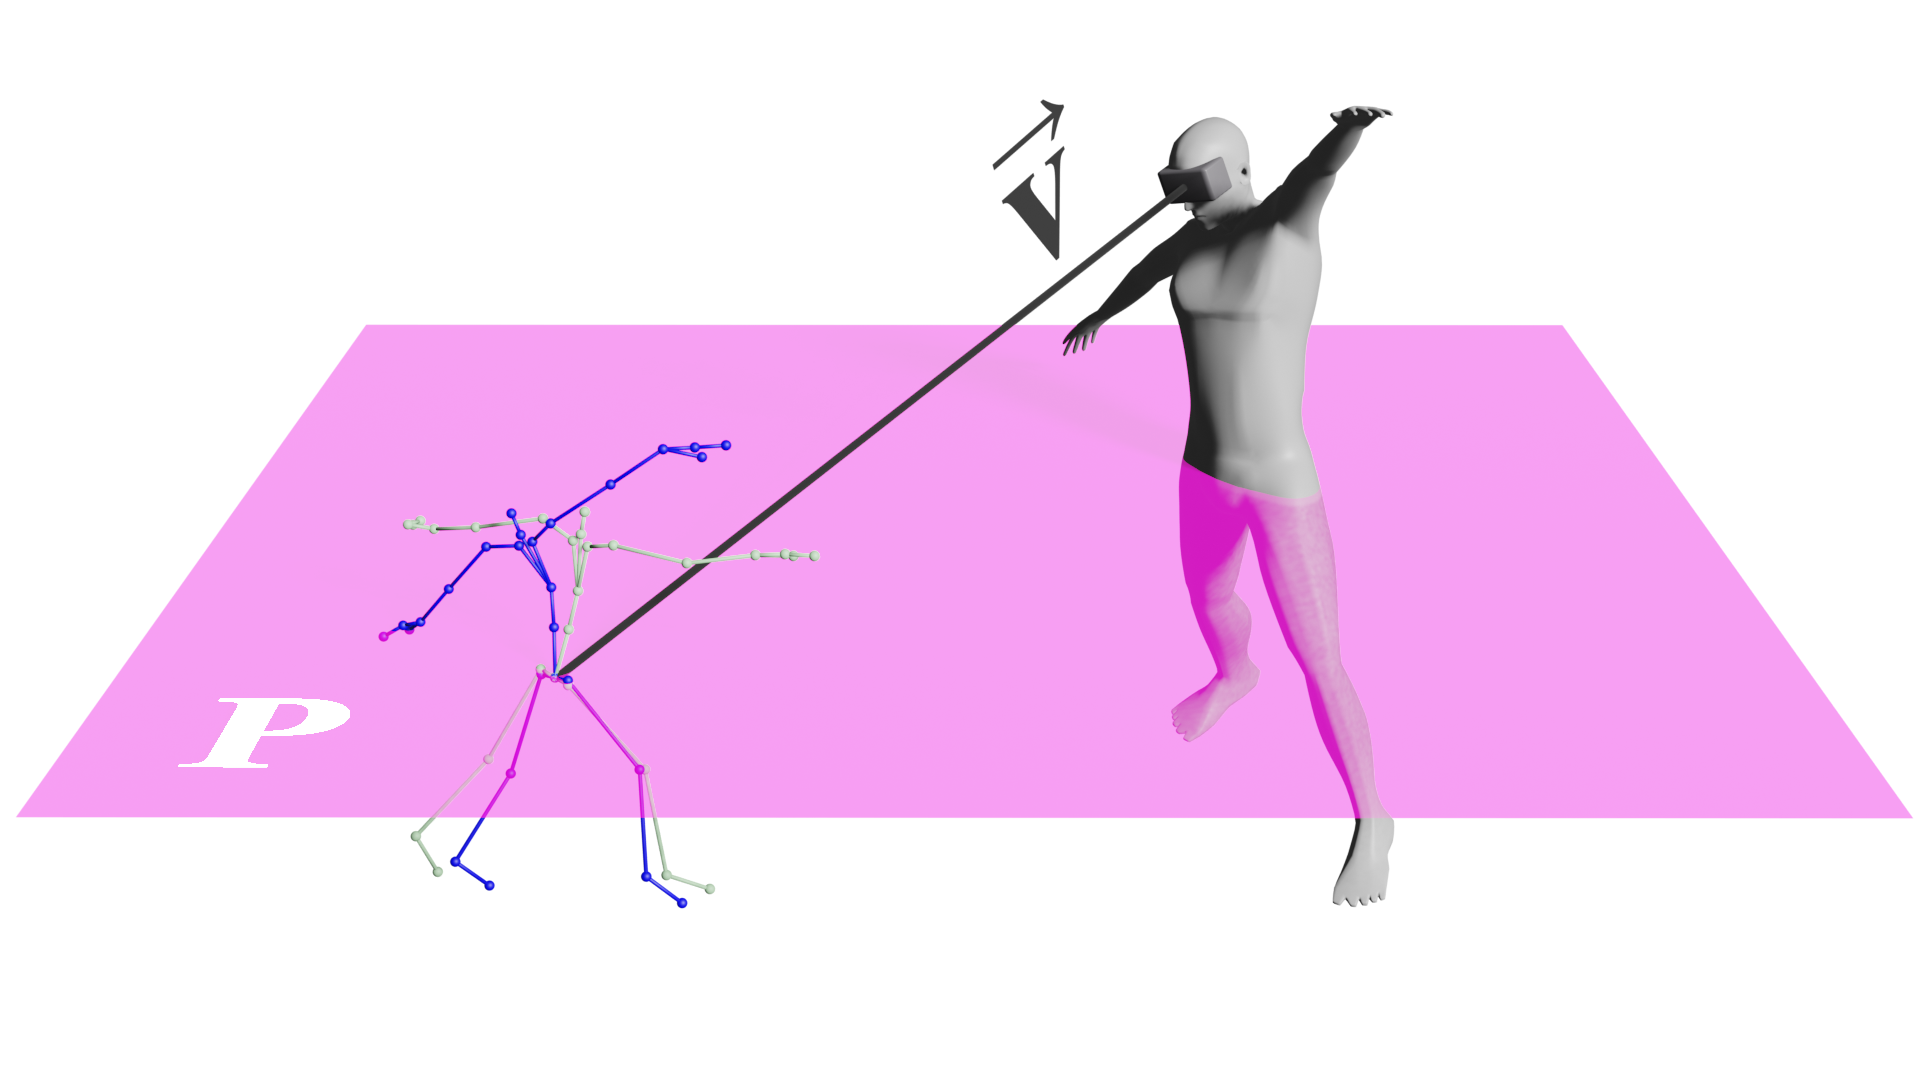
\includegraphics[width=0.6\linewidth]{pictures/avatarPos.png}
	\caption[Positioning of the feedback avatar.]{The feedback avatar is positioned such that its pelvis lies on the intersection of the view direction $\vec{v}$ and the horizontal plane through the user's pelvis $P$.\label{fig:positioning}}
\end{figure}

\textbf{Snapping:}
While moving --- especially during exercises --- the head movement can be unstable, leading to an erratic feedback placement. Consequently, the visual feedback becomes irritating for the user. Therefore SkillAR only moves the feedback if the intersection of $\vec{v}$ with $P$ exceeds a certain distance $\Delta$ from the current avatar position as seen in~\autoref{fig:roundGrid}. The feedback is moved smoothly to its new position, which leads to a far more stable system behavior similar to snapping.

\begin{figure}[t!]
	\centering
	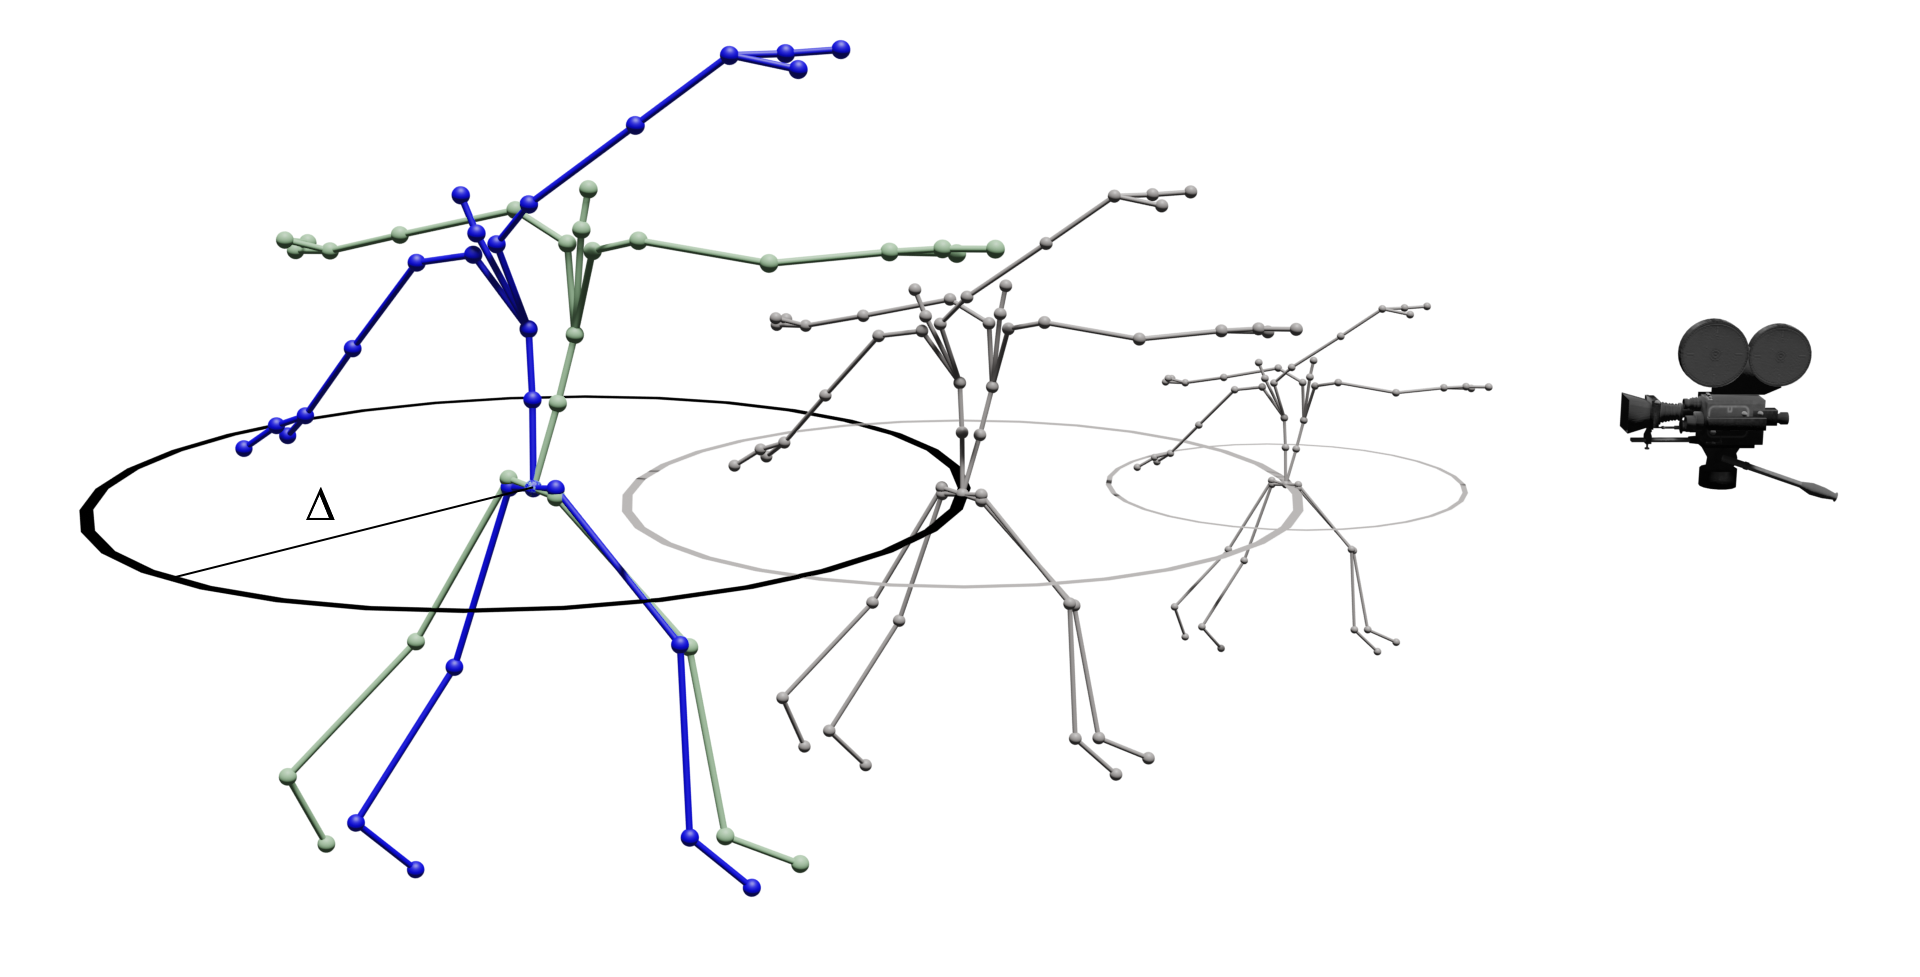
\includegraphics[width=0.6\linewidth]{pictures/gridRound.png}
	\caption[Spatial stabilization of the feedback positioning.]{The avatars move horizontally if the view direction deviates more than $\Delta$ from the center of the visualization, as indicated by the circles. The visualization is scaled up in the distance and down in proximity to the camera. The constant size always matches the field of view of the \acrshort{hmd} and irritates the user less as if it were constantly changing.\label{fig:roundGrid}}
\end{figure}

\textbf{Scaling:}
Moreover, the size of the feedback is scaled depending on the distance to the virtual camera to optimally utilize the \acrshort{hmd}'s field of view.  This is illustrated in~\autoref{fig:roundGrid}. Likewise, the snapping threshold $\Delta$ is scaled (also visible in~\autoref{fig:roundGrid}) to facilitate a consistent user interaction. Scaling the avatar results in slightly contradicting depth cues: The vergence changes with the distance, but the size stays constant due to the scaling. Additionally, the avatars are still appropriately located in the scene, but they might no longer connect with the real floor plane. However, it is to be said, that our priority is to provide omnipresent in-situ feedback rather than creating a perfectly immersive experience. None of the users commented about the above-mentioned topics (see \autoref{sec:comments}).

\textbf{Top-Down Mode:}
When looking down, the feedback positioning at pelvis height becomes hard to perceive as it appears too close. This would prevent the user from perceiving feedback when doing exercises that involve a downward head orientation like planks or push-ups. For this reason, when the angle $\gamma$ between the view direction $\vec{v}$ of the \acrshort{hmd} and the vertical axis lies below 20° (see in~\autoref{fig:floor}), SkillAR displays the feedback in a constant distance below the user (underneath the physical floor plane). In this top-down view, the avatars are facing the same way as the user and are not mirrored. This provides an overview of exercises facing down, allowing for an \acrshort{ar}-supported execution of, for example, push-ups.

\begin{figure}[h!]
	\centering
	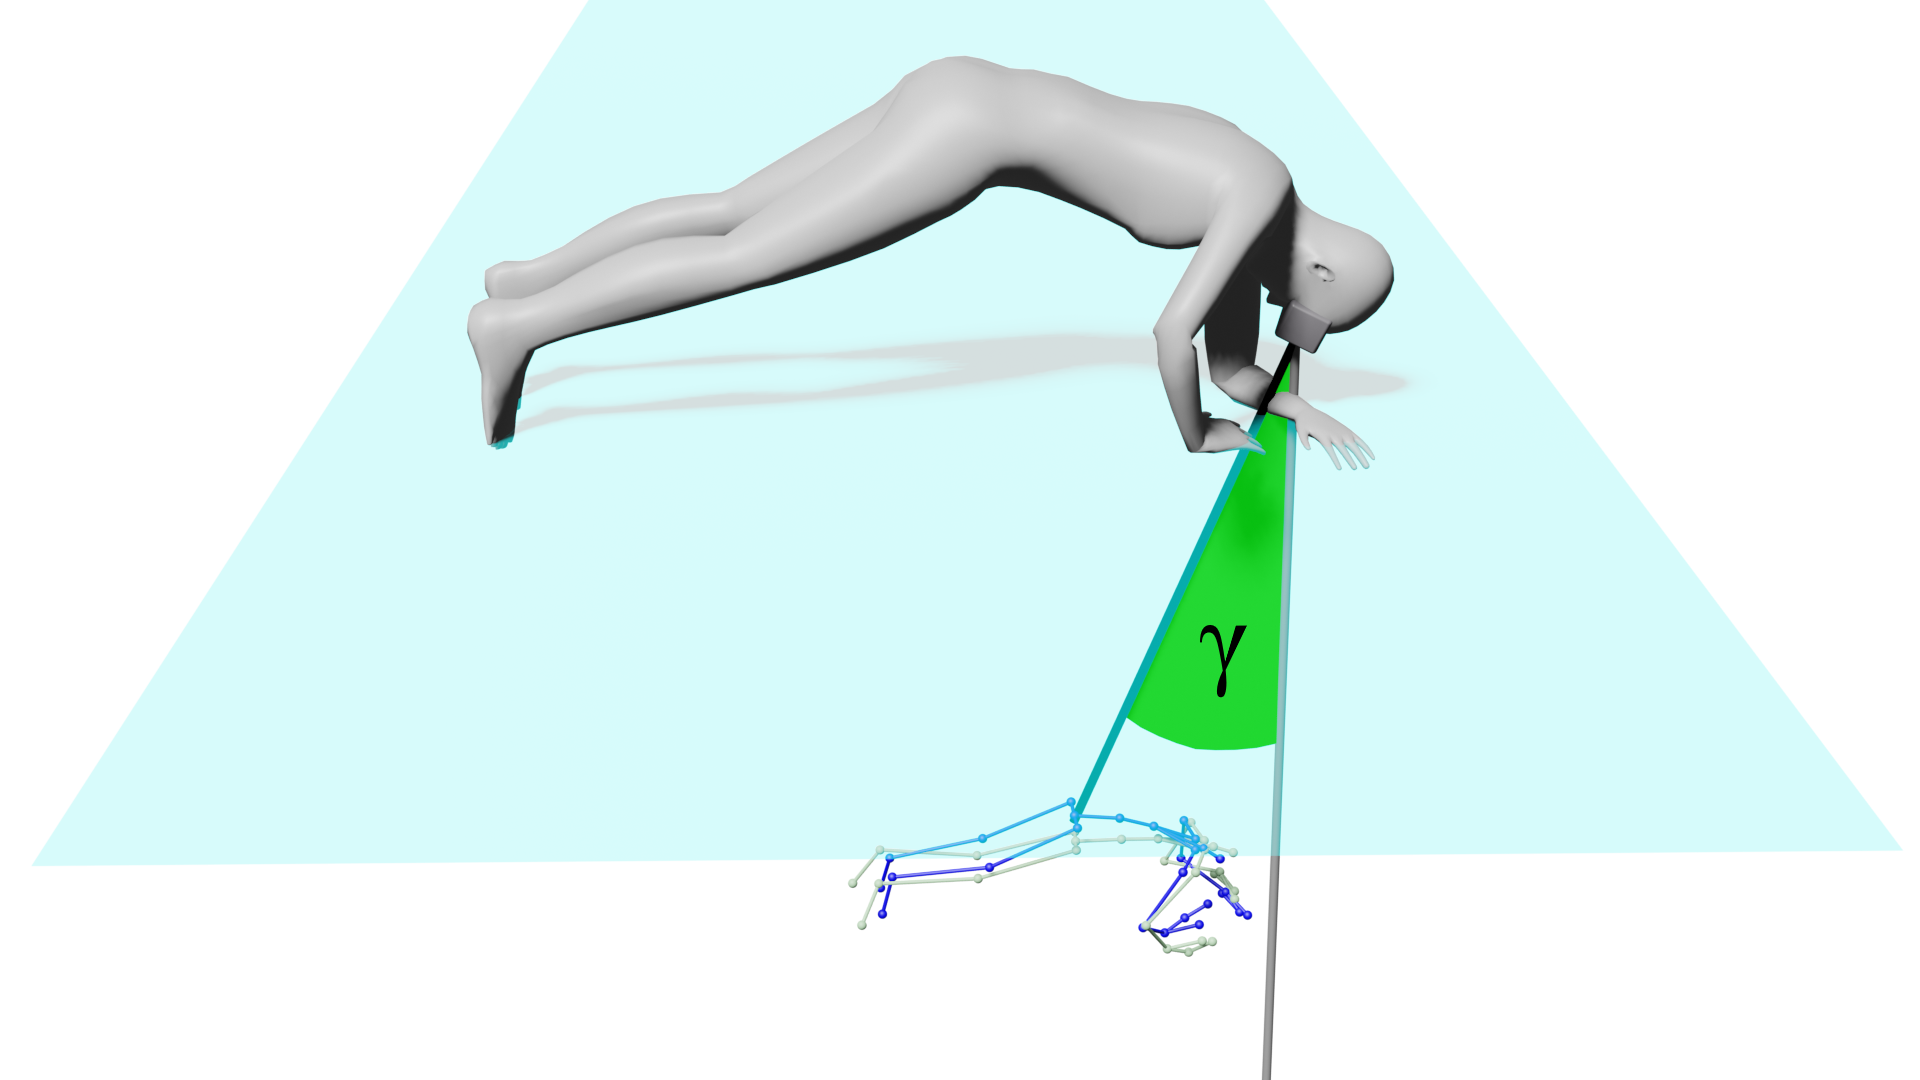
\includegraphics[width=0.6\linewidth]{pictures/floorPos.png}
	\caption[Top-down mode visualizing exercises when looking down.]{The feedback transitions to a \emph{top-down mode}, in which the avatars are shown below, if the angle $\gamma$ between the normal of the floor and the view direction is smaller than 20°. \label{fig:floor}}
\end{figure}

\textbf{Free Mode:}
Likewise, the feedback positioning mode changes when looking upwards. In this case, the avatars can not be placed at the intersection of $\vec{v}$ and $P$ as they no longer intersect. Consequently, the avatar positioning is then strictly bound to the view direction. The distance to the camera is constant, and the avatar still faces the user. While the avatar's relation to its environment is less clear in this mode, it allows for performing exercises with an upward-facing view direction like sit-ups or bench press.

\section{Evaluation}
SkillAR provides major advantages for viewing motor feedback: Users can view the ideal form while performing exercises without compromising comfort, good form, or safety. We conducted a user study to verify that SkillAR has no additional major disadvantages compared to a conventional \acrshort{rmd}. This study was reviewed by the ethics committee and the data protection official of the University of Applied Sciences Worms and carried out following the appropriate guidelines and regulations. Consequently, the participants were informed upon invitation about the legal circumstances and anonymity of the study. Only the following data was recorded: Age, gender, vision deficiencies, and affiliation with the university. It is not feasible, that they lead to identifying a person's identity. Therefore, written consent was not necessary according to the ethics committee and data security office. \acrshort{usb} drives and sunglasses were offered as compensation.

\subsection{Participants}
For the user study, 32 individuals were recruited from an academic environment. Their age ranged from 22 to 61 (\(\mathrm{M} = 35.4, \mathrm{Mdn} = 30.5, \mathrm{SD} = 11.1\)). Their gender was evenly distributed among males and females with 16 (\(50.0\%\)) individuals each. They rated their prior \acrshort{xr} experience on a scale from one to five, with one equaling no previous engagement in \acrshort{xr} and five being an \acrshort{xr} expert. The rating averaged out at 1.8 (\(\mathrm{M}=1.8, \mathrm{Mdn} = 1.75, \mathrm{SD} = 0.9\)) and their physical activity at 3.1 (\(\mathrm{M}=3.1, \mathrm{Mdn} = 3, \mathrm{SD} = 0.9\)) (one again representing no physical activity and five the maximum). As the visual capabilities of individuals play an important role in the study, the number of participants wearing glasses (\(\mathrm{n} = 17, \mathrm{i.e.}~53.1\%\)) was documented as well as visual impairments: Three participants (\(9.4\%\)) reported to have limited or missing spatial perception. One participant exhibited both red-green and blue-yellow color vision deficiency. Regarding gender, the participants' demographics match the population of Europe and the world well. The median age of the participants lies between the median age of Europe (\(42.2\)) and the world (\(30.4\)) as estimated by the \acrshort{un} in 2023~\cite{united2022world}. However, the educational background is expected to be higher than average in our user group, as the individuals were recruited in an academic environment.


\subsection{Apparatus}
A Microsoft Azure Kinect 3D camera provided the spatial positions of the joints. It was set up on a tripod about 2,5 m from the subject to ensure that everything was in frame. The visualization and experimental applications were developed in Unity. To display the augmented reality sections of the study a Microsoft HoloLens 2 was utilized. Additionally, to ensure the legibility on the HoloLens, the blinds in the room were closed to provide consistent lighting conditions for the participants. Internal pilot studies showed, that it is hard to perceive the visualization in intensely illuminated environments.

It was ensured the participants understood the avatars, the visual feedback, and the study tasks beforehand. The study took a total of about 20 min with 5 min of introduction. Every task demanded approximately the same duration. Exercises could be skipped or aborted at any time due to health concerns.

\subsection{Tasks \label{sec:tasks}}
In the \textbf{comparison} task, the user was asked to identify errors represented by an actual and a target avatar as seen in \autoref{fig:exercises}. The answers were documented and categorized, regarding the accuracy of the addressed body part and correction. With both --- the body part and the correction --- being able to be either correct or incorrect, this led to $2 \times 2$ categories. It was possible for answers to fall into several categories, as sometimes participants made contradicting remarks or answered both correctly and incorrectly successively. Additionally, the time to answer was measured. This task was carried out using the \acrshort{hmd} and the \acrshort{rmd} sequentially.

The \textbf{imitation} task involved the users mimicking a pose they saw superimposed with their actual pose on the \acrshort{hmd} or \acrshort{rmd}. After adapting the pose, they gave a command, and the distances of joints, and the time elapsed since the display started showing the pose, were recorded. In between the exercises, no feedback was visible, and the users could retake a neutral position and recover from the previous exercise. This should prevent impacting the following exercise performances in any way (e.g. adding time, because the participant has to stand up after an exercise on the ground). This task was carried out using the \acrshort{hmd} and the \acrshort{rmd} sequentially.

Finally, the participants answered structured \textbf{questions} regarding their demographic including age, affiliation, XR experience, physical activity, optical deficiencies, gender, and potential comments.

\subsection{Study Design \label{sec:design}}
The study aimed to compare SkillAR to conventional \acrshort{rmd}s using an in-subject design measuring time and accuracy during the comparison and identification tasks. A few border case exercises were selected, representing various body positions in space. In addition, deviations were chosen to be evaluated during the comparison task (see below) to evaluate the feedback interpretation. These deviations require corrections in different directions to correct: Bend vertically, tilt side-wards, raise or lower limbs, twist, etc. Furthermore, the following exercises were each represented by a still pose: Standing, jumping jack, plank, squat, torso rotations, and warrior II as found in yoga. These exercises can be seen including the deviations from the ideal in \autoref{fig:exercises}. The order of exercises, tasks, and devices was randomized to eliminate any learning bias. Moreover, the intent of the study was not to evaluate how well an exercise was executed, but how well the feedback could be comprehended.

In the \textbf{comparison} task, users were asked to identify errors represented by an actual and a target avatar as seen in \autoref{fig:exercises}. The answers were documented and categorized, regarding the accuracy of the addressed body part and correction. With both --- the body part and the correction --- being able to be either correct or incorrect, this led to $2 \times 2$ categories. It was possible for answers to fall into several categories, as sometimes participants made contradicting remarks or answered both correctly and incorrectly successively. Additionally, the time to answer was measured. This task was carried out using the \acrshort{hmd} and the \acrshort{rmd} sequentially.

The \textbf{imitation} task involved the users mimicking an ideal pose they saw superimposed with their actual pose on the \acrshort{hmd} or \acrshort{rmd}. After adapting the pose, they gave a command, and the distances of joints, and the time elapsed since the display started showing the pose, were recorded. In between the exercises, no feedback was visible, and the users could retake a neutral position and recover from the previous exercise. This should prevent impacting the following exercise performances in any way (e.g. adding time, because the participant has to stand up after an exercise on the ground). This task was again carried out using the \acrshort{hmd} and the \acrshort{rmd} sequentially. The supplemental material provides a video of the juxtaposed exocentric and egocentric perspectives of a user imitating poses.

Finally, the participants answered structured \textbf{questions} regarding their demographic including age, affiliation, \acrshort{xr} experience, physical activity, optical deficiencies, gender, and potential comments.

\section{Results}
We suspected a dependency between \acrshort{rmd} and \acrshort{hmd} regarding the results of the same tasks. Additionally, we had no assumption which device would allow for more accuracy or a faster task completion time. Consequently, a dependent two-tailed t-test seemed most appropriate to evaluate the results. For this purpose, the results of one individual were averaged, so they were comparable during the test. One evaluation of the comparison task was discarded, as it was not suitable for evaluation due to technical difficulties leading to an incomplete recording. For the t-test, we assumed a significance level of \(\mathrm{\alpha} = 0.05\).

\subsection{Completion Time Analysis}
During each of the study tasks, the time to completion was measured. In particular, the time from the start of displaying the exercise to identifying the exercise or adopting the displayed pose. When imitating poses, this was starting from a neutral standing pose.

\begin{table}[b!]
	\caption{Time measurements for each task in the user study.}\label{tab:time}
	\begin{tabular*}{\textwidth}{@{\extracolsep\fill}lcccccc}
		\toprule%
		& \multicolumn{2}{@{}c@{}}{Comparison} & \multicolumn{2}{@{}c@{}}{Imitation} \\\cmidrule{2 - 3}\cmidrule{4-5}%
		Device & \acrshort{rmd} & SkillAR & \acrshort{rmd} & SkillAR \\
		\midrule
		Mean  & 18.81 s & 19.01 s & 21.42 s & 22.95 s\\
		Median & 14.70 s  & 17.95 s  & 19.94 s & 22.43 s\\
		Standard Deviation  & 11.44 s & 8.17 s & 7.78 s & 7.80 s\\
		\bottomrule
	\end{tabular*}
\end{table}

Regarding the comparison task, SkillAR exhibits an insignificantly (\(\mathrm{p}=0.92\)) longer time to assess the feedback while featuring a lower standard deviation, as seen in \autoref{tab:time}. Likewise, the users required an insignificantly (\(\mathrm{p}=0.38\)) longer time to mimic the poses displayed with SkillAR compared to the \acrshort{rmd}.

\subsection{Accuracy Analysis}
In the comparison task, the percentage of right answers (right body part and right correction) was recorded per user per device. When measuring the accuracy of the pose imitation, we measured the distance of each joint to its counterpart in the ideal pose. These were then averaged to find the mean deviation of the user pose per device.

Assessing the accuracy in the comparison task between the \acrshort{rmd} and SkillAR, we see
that users could identify the corrections significantly (\(\mathrm{p}=6 \cdot 10^{-7}\)) more precisely with SkillAR in relation to a conventional \acrshort{rmd}. As in this case the p-value is far smaller than $\alpha$, it seems likely that SkillAR facilitates a more precise interpretation of the given feedback. When imitating the poses, the precision was insignificantly (\(\mathrm{p}=0.37\)) higher using the \acrshort{rmd} compared to SkillAR.


\begin{table}[b!]
	\caption{Accuracy for each task in the user study.}\label{tab:accuracy}
	\begin{tabular*}{\textwidth}{@{\extracolsep\fill}lcccccc}
		\toprule%
		& \multicolumn{2}{@{}c@{}}{Comparison} & \multicolumn{2}{@{}c@{}}{Imitation} \\\cmidrule{2 - 3}\cmidrule{4-5}%
		Device & \acrshort{rmd} & SkillAR & \acrshort{rmd} & SkillAR \\
		\midrule
		Mean  & 75.27 \% & 92.71 \% & 10.71 cm & 11.14 cm\\
		Median & 83.33 \% & 100.00 \% & 10.17 cm & 10.82 cm\\
		Standard Deviation  & 11.88 \% & 12.46 \% & 2.56 cm & 3.33 cm\\
		\bottomrule
	\end{tabular*}
\end{table}

\section{Discussion}
In the statistical analysis, we could not verify a significant difference between SkillAR and \acrshort{rmd} regarding the comparison time as well as time and accuracy when mimicking poses. The large standard deviation compared to the mean suggests that an even more controlled study with more participants and a more precise camera could be profitable. Further, the measurements of the two analyzed methods seem quite similar. It might be profitable to analyze the statistical equivalence of the methods in future studies. However, our evaluation shows that the participants identify the right feedback significantly more often with SkillAR compared to an \acrshort{rmd}. The mean difference is large compared to the standard deviation. We attribute this mainly to the fact, that it is possible to perceive a 3D image of the feedback with the \acrshort{hmd}: Due to the two displays in the \acrshort{hmd}, a stereoscopic image is created. This represents an additional depth cue compared to the screen. The adaptive nature and the positioning of the feedback in the room could further enhance the interpretation of the scene. Lastly, the rotation of the avatar to the user as described in \autoref{sec:transformation} reduces motion parallax, but it still could be a factor when the feedback is moved away and towards the user.

Additionally, our approach provides the major advantage of an independent viewing direction. This facilitates in-situ feedback in many situations where it otherwise would be inconvenient with a conventional \acrshort{rmd} or impossible. Furthermore, the independent head direction enables the user to perform exercises optimally.
\subsection{User Comments \label{sec:comments}}
After the study, the users were asked if they had comments concerning the system. Eleven participants stated that it was easier to perceive the feedback and execute the poses with SkillAR. This happened without being prompted to compare the conventional \acrshort{rmd} and SkillAR. The remarks match our findings when evaluating the accuracy with which the feedback was identified with SkillAR. Similarly, this could be attributed to the additional depth perception in \acrshort{ar}. In contrast, only one person preferred the feedback on the \acrshort{rmd}, as they disliked the feedback adapting to the head movement altogether in SkillAR. Moreover, some users reported understanding the poses not until using SkillAR. This was never observed the other way around and also matches the previous findings.

Additionally, three people reported that they recognized a discrepancy between how they remembered to do the exercise right and what they saw. One of these participants reported neglecting the experience with the exercise and relied completely on the visualization. This emphasizes how careful exercise feedback must be considered. If the visualization can override motor perception, it is crucial to ensure the feedback is safe for the user.

Furthermore, the participants with limited spatial perception or color vision deficiency reported that they had no problems regarding their deficiencies when using the system.

\subsection{Observable Behaviors \label{sec:behaviors}}
In addition to the answers and comments of the users, there were interesting behaviors that could be observed multiple times during the study. For instance, where possible, some participants used the \acrshort{hmd} like a conventional \acrshort{rmd}: Always looking at the same spot, although the view direction could be arbitrary. Additionally, many users did not utilize the \emph{top-down viewing mode} for the planks as explained in~\autoref{sec:transformation}. These observations led us to the conclusion that our system could be leveraged even more with more extensive instructions, explaining the full functionalities of SkillAR. Furthermore, this could lead to interesting new research analyzing the reason for these behaviors and the possible consequences, especially regarding deviations from the ideal execution.

Moreover, when adopting a pose, the users predominantly preferred to correct one limb after another --- in some cases, the lower and upper body separately. This could be important to consider in the future when providing visual feedback for several deviations at once. Additionally, the registration of the avatars as explained in~\autoref{sec:register} seemed to yield potential for optimization in some cases. For particular, users tried to adapt their pose by rotating in space, although the avatar was always facing the (virtual) camera. The selection of registration methods for this application could be reevaluated. This highlights once more the important nature of registration and its impact on user experience. For more detail on registration methods see \autoref{chap:registration}.

\subsection{Limitations}
Although our system provides major advantages for in-situ motor feedback, some limitations must be mentioned. For instance, some exercises or sports are difficult to combine with an \acrshort{hmd}. In particular, exercises where the head has to rest on the floor might be uncomfortable or impossible to do, due to the headset interfering. Similarly, the same is true for exercises that involve contact with the head (e.g. pulling on the head for neck stretching). Additionally, some sports might not be suited for an augmentation with an \acrshort{hmd} or require technology tailored to the situation. For example, swimmers might require a special waterproof \acrshort{hmd} to receive similar feedback. Likewise, sports that require a helmet --- like American football or ice hockey --- could require a special \acrshort{hmd} built into the helmet. Due to the limited robustness featured by standard \acrshort{hmd}s, they might not be fit for a sport with forces applied to the head area. Furthermore, the 3D camera we used to record the users' joint positions in space is not precise enough to detect very delicate movements. Therefore, it would be beneficial to assess the topic with a more precise motion tracking system in the future. Lastly, rotating the avatars to face the virtual camera as described in~\autoref{sec:transformation} reduces motion parallax as a depth cue. This could limit the interpretation of the feedback. Especially individuals with limited spatial perception could be impaired by this, as they might not be able to profit from other depth cues.

\section{Conclusion}
The chapter at hand presents a novel method to provide omnipresent in-situ motor feedback. It does not only provide feedback where it would be otherwise not possible, but it also enables the user to perform exercises more correctly, more comfortably, and in a non-injurious manner. Additionally, we conducted a user study including 32 participants. We could not detect a significant difference between SkillAR and conventional \acrshort{rmd} in terms of identification, imitation time, and imitation accuracy. Moreover, the study showed that the users could identify the errors more accurately when receiving feedback via SkillAR. Thus, we can conclude that our method bears major advantages in contrast to feedback via a conventional \acrshort{rmd}, as exercise execution and comfort are not compromised and feedback can be provided independently of the head position.

\section{Future Work}
As discussed in~\autoref{sec:behaviors}, we developed a comprehensive framework for registration of superimposed avatars, as presented in \autoref{chap:registration}. It might be beneficial for user experience to reassess the registration methods used in SkillAR. Additionally, repeating the experiments using a more controlled environment could lead to the detection of minor effects that were beyond the scope of this paper.

Moreover, the present findings provide a foundation for further research. Future approaches could explore the potential of the system with a more comprehensive user introduction, explaining all the capabilities and using it in a more exhaustive training scenario. With the fundamentals assessed, it will be valuable to assess the system performance with further poses or when doing dynamic exercises.

Additionally, it might be interesting to extend SkillAR with automatic viewpoint selection methods as presented in \autoref{chap:viewpoint}. This could further facilitate feedback understanding. For example, in top-down mode, where the comprehension of the vertical posture of the spine is mostly limited to stereoscopic depth cues.